% Preamble.
\documentclass{article}

\title{Programming Project 6}
\author{Max Reilly, copied from Hanly and Koffman}
\date{August 7, 2025}

\usepackage{pdfpages}
\usepackage{graphicx}

\begin{document}
    \maketitle
    \section{Assignment}
    You would like to find the area under the curve
    \begin{equation}
        y = f(x)
    \end{equation}
    between the lines $x = a$ and $x = b$. One way to approximate this area is to use
    line segments as approximations of small pieces of the curve and then to sum
    the area of trapezoids created by drawing perpendiculars from the line segment
    endpoints to the $x$-axis, as shown in Fig. 7.13. We will assume that $f(x)$
    is non-negative over the interval $[a,b]$. The trapezoidal rule approximates
    this area $T$ as
    \begin{equation}
        T = \frac{h}{2} \left(f(a) + f(b) + 2 \sum^{n-1}_{i = 1} f(x_i)\right)
    \end{equation}
    for $n$ subintervals of length $h$:
    \begin{equation}
        h = \frac{b - a}{n}
    \end{equation}
    Write a function \verb|trap| with input parameters \verb|a|, \verb|b|, \verb|n|, and \verb|f| that
    implements the trapezoidal rule. Call \verb|trap| with values for \verb|n| of 2, 4, 8, 16, 32, 64,
    and 128 on functions
    \begin{equation}
        g(x) = x^2 sinx \qquad (a = 0, b = 3.14159)
    \end{equation}
    and
    \begin{equation}
        h(x) = \sqrt{4 - x^2} \qquad (a = -2, b = 2)
    \end{equation}
    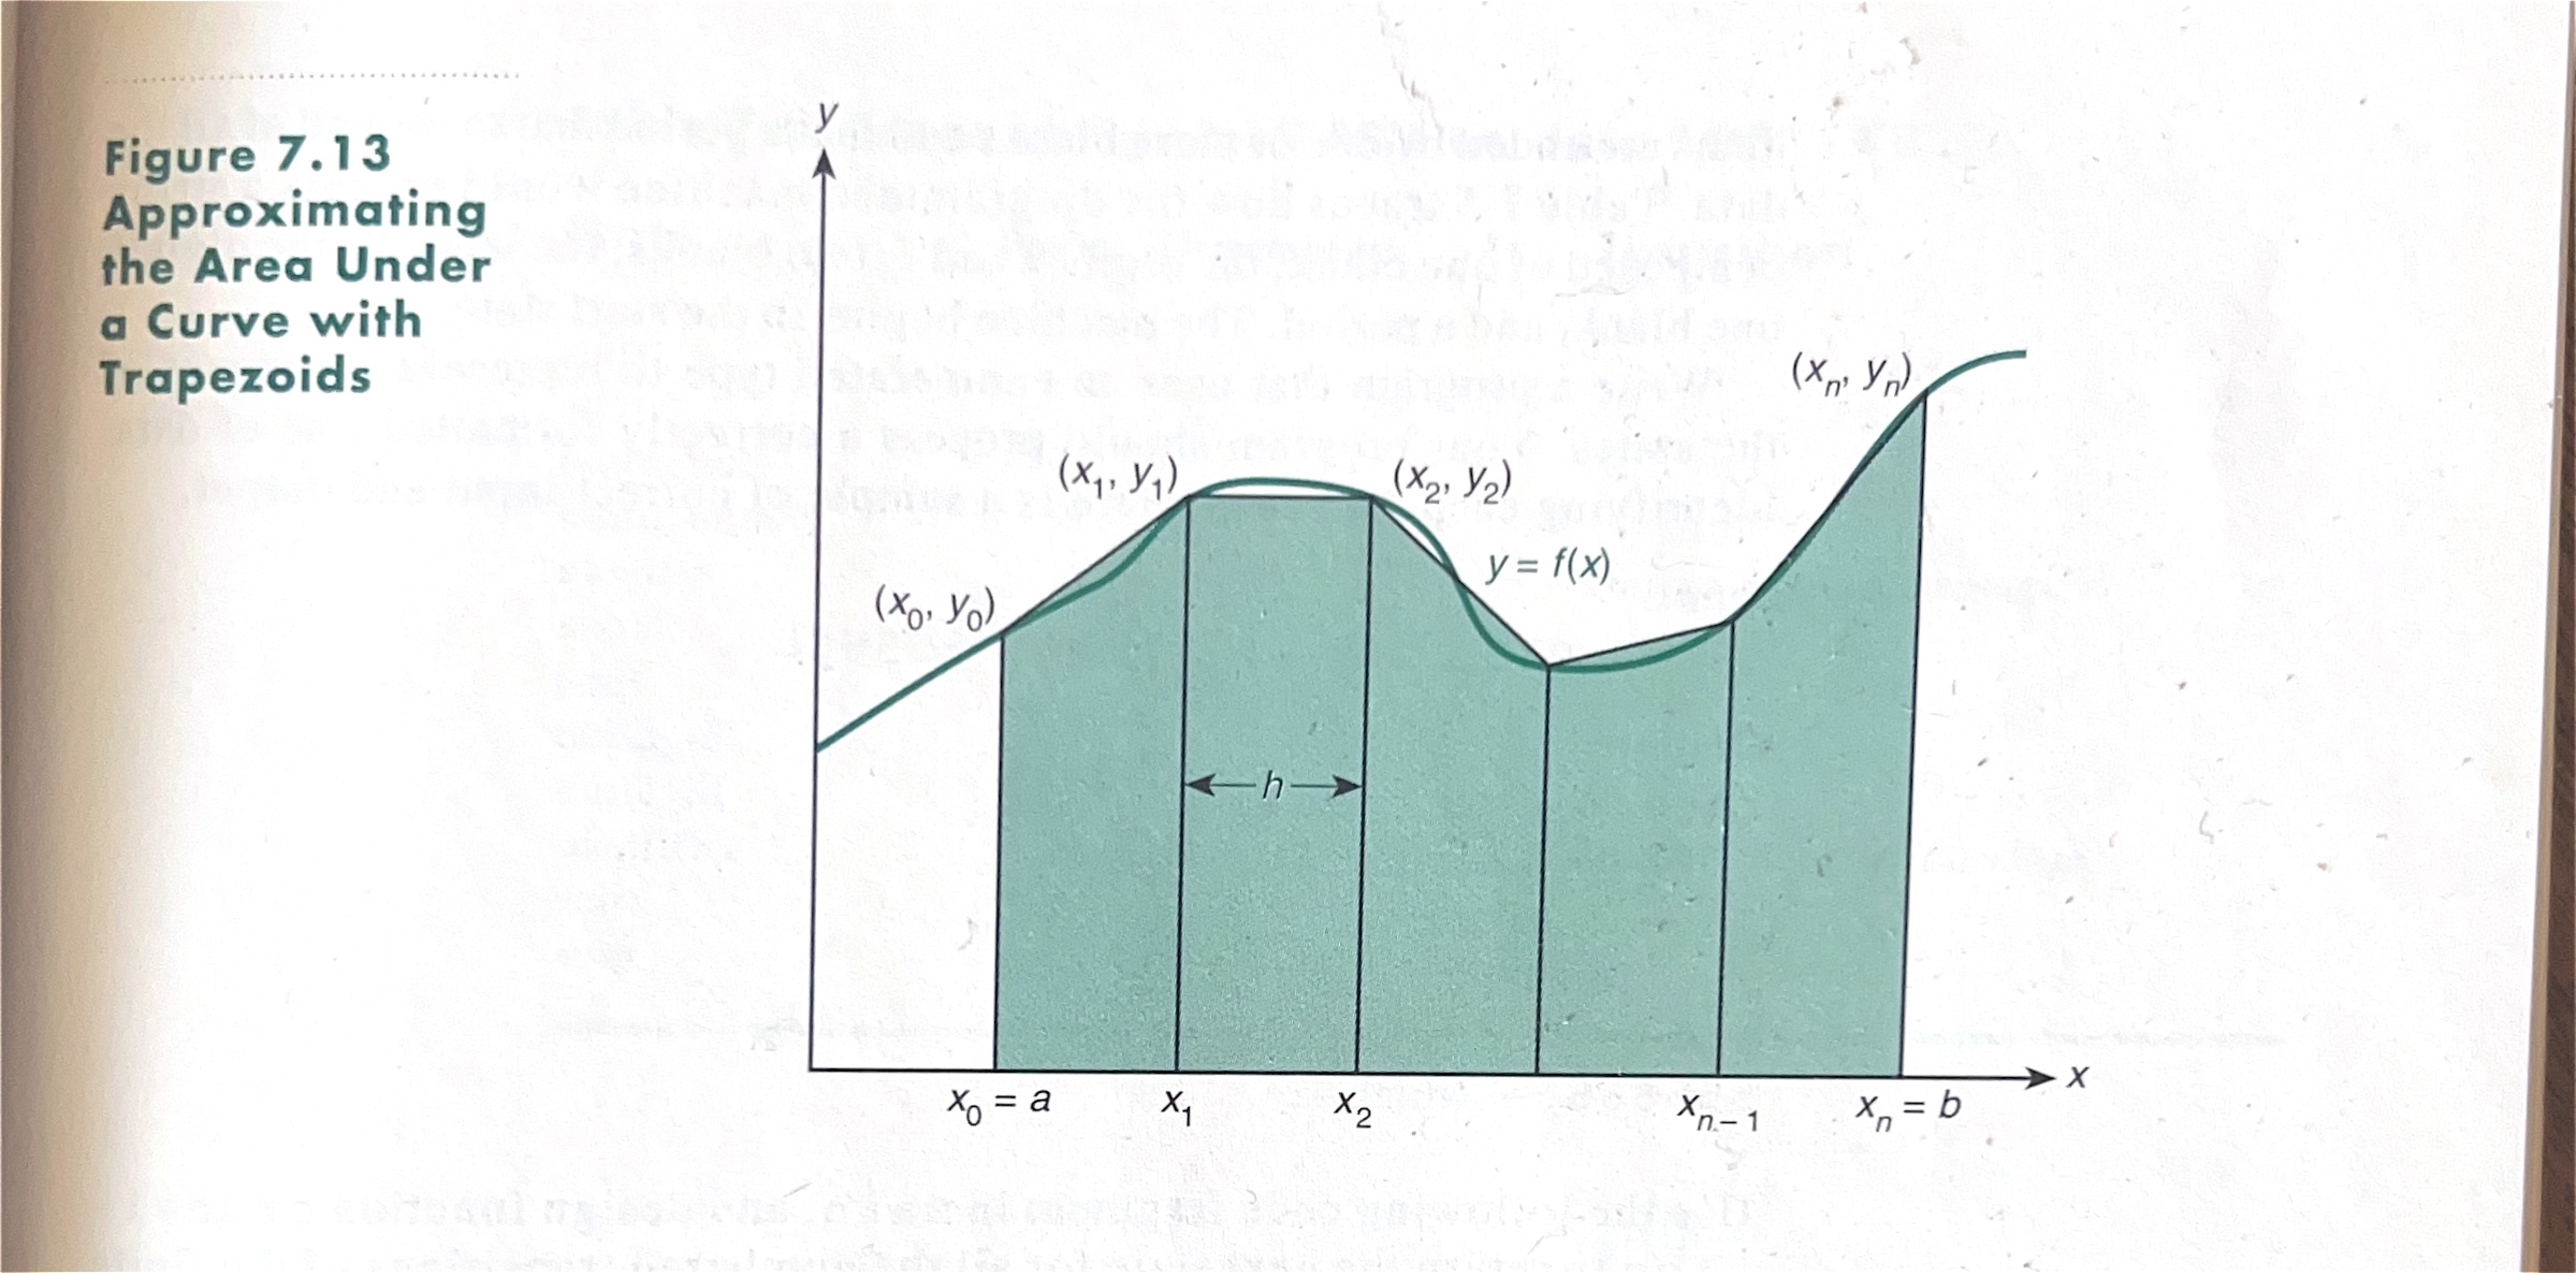
\includepdf[pages=-]{hk7.13.pdf}
    Function $h$ defines a half-circle of radius 2. Compare your approximations to
    the actual area of this half circle.

    {\em Note:} If you have studied calculus, you will observe that the trapezoidal
    rule is approximating
    \begin{equation}
        \int_{a}^{b} f(x)dx
    \end{equation}

\end{document}
